\documentclass[a4paper]{article}
\usepackage[utf8]{inputenc} % Skal passe til editorens indstillinger
\usepackage[english]{babel} % danske overskrifter


\newcommand{\name}{Carsten Nielsen}
%\newcommand{\stnumber}{s123369, s123161, s123821}
\newcommand{\course}{INI 404 Neuromorphic Engineering~I}
\newcommand{\university}{University of Zürich}
\newcommand{\studyline}{Institute of Neuroinformatics}
\newcommand{\assignment}{Lab 8 Post-Lab}
\renewcommand{\date}{\today} %If another date, than that of today is desiered


% Palatino for rm and math | Helvetica for ss | Courier for tt
\usepackage{mathpazo} % math & rm
\linespread{1.05}        % Palatino needs more leading (space between lines)
\usepackage{palatino} % tt
\normalfont
\usepackage[T1]{fontenc}
\usepackage[english]{babel}

\usepackage{graphicx}%allerese hentet % indsættelse af billeder
\usepackage{epstopdf} %Tilfj "--enable-write18" i argumentet for LaTex build. Dette vil konvertere .eps figurer til pdf-format
\graphicspath{{./picture/}} % stivej til bibliotek med figurer
\usepackage{subcaption} %Til gruppering af figurer
\usepackage{amsmath} %matpakke
\usepackage{amsfonts} %
\usepackage{amssymb} %
\usepackage{steinmetz} % flere matematik symboler
\usepackage{polynom} %for displaying polynom division
\usepackage{mathtools} % matematik - understøtter muligheden for at bruge \eqref{}
\usepackage{float}
\usepackage{placeins}
\usepackage{hhline}

%
\usepackage[usenames,dvipsnames]{xcolor}
\usepackage[compact,explicit]{titlesec}% http://ctan.org/pkg/titlesec
%
\usepackage[europeanresistors]{circuitikz}
\usepackage{pgfplots}
\usepgfplotslibrary{patchplots}
\pgfplotsset{compat=1.11}

%---------%
%Easy edit%
%---------%

%Section formating. arg1 is supplied when making section
\newcommand\presectionnumber[1]{~~}
\newcommand\postsectionnumber[1]{}
\newcommand\midlesection[1]{#1}
\newcommand\sectionnum[1]{\arabic{#1}}
\newcommand\subsectionnum[1]{\arabic{#1}}
\newcommand\subsubsectionnum[1]{\alph{#1}}



%------------%
%setion setup%
%------------%
\renewcommand\thesection{Opgave~\sectionnum{section}} %pas p�, kun i matematik
\renewcommand\thesubsection{\thesection,~\subsectionnum{subsection}}
\definecolor{MagRed}{RGB}{190,40,15}
\definecolor{MathGreen}{RGB}{82,164,0}

\titleformat{\section}{\normalfont\sffamily\large\bfseries\color{MathGreen}}{}{0pt}{|\kern-0.15ex|\kern-0.15ex|\kern-0.15ex|\presectionnumber{#1}\sectionnum{section}\postsectionnumber{#1}\qquad\quad\midlesection{#1}\label{sec:\sectionnum{section}}}
\titleformat{\subsection}[runin]{\large\bfseries}{}{10pt}{\sectionnum{section}.\subsectionnum{subsection})~#1\label{sec:\sectionnum{section}.\subsectionnum{subsection}}}
\titleformat{\subsubsection}[runin]{\itshape}{}{0pt}{\subsectionnum{subsection},\subsubsectionnum{subsection}~#1\label{sec:\sectionnum{section}.\subsectionnum{subsection}.\subsubsectionnum{subsubsection}}}
%\titleformat{\subsubsection}{\bfseries}{}{0pt}{\alph{subsection}.\arabic{subsubsection})\qquad\quad#1\label{\arabic{section}\alph{subsection}\arabic{subsubsection}}}

%----------%
%page setup%
%----------%
\textwidth = 400pt
\marginparwidth = 86pt
\hoffset = -25pt
\voffset= -30pt
\textheight = 670pt

%--------%
%hyperref%
%--------%
\newcommand{\HRule}{\rule{\linewidth}{0.5mm}}
\usepackage{fancyhdr}
\usepackage[plainpages=false,pdfpagelabels,pageanchor=false]{hyperref} % aktive links
\hypersetup{%
  pdfauthor={\name},
  pdftitle={\assignment},
  pdfsubject={\course} }
%\usepackage{memhfixc}% rettelser til hyperref

%-------------%
%Headder setup%
%-------------%
\fancyhf{} % tom header/footer
\fancyhfoffset{20pt}
\fancyhfoffset{20pt}
\fancyhead[OL]{\name \\ INI 404}
\fancyhead[OC]{Date \\ \date}
\fancyhead[OR]{\university\\ \studyline}
\fancyfoot[FL]{}
\fancyfoot[FC]{\thepage}
\fancyfoot[FR]{}
\renewcommand{\headrulewidth}{0.4pt}
\renewcommand{\footrulewidth}{0.4pt}
\headsep = 35pt
\pagestyle{fancy}
 % style setup

%Listings%
\usepackage{listingsutf8}
\usepackage[framed,numbered]{matlab-prettifier}


%setup listings
\lstset{language=Matlab,
  extendedchars=true,
  language=Octave,                % the language of the code
  basicstyle=\ttfamily\footnotesize,           % the size of the fonts that are
  % used for the code
  numbers=left,                   % where to put the line-numbers
  numberstyle=\tiny\color{gray},  % the style that is used for the line-numbers
  stepnumber=2,                   % the step between two line-numbers. If it's 1, each line 
                                  % will be numbered
  numbersep=5pt,                  % how far the line-numbers are from the code
  backgroundcolor=\color{white},      % choose the background color. You must add \usepackage{color}
  showspaces=false,               % show spaces adding particular underscores
  showstringspaces=false,         % underline spaces within strings
  showtabs=false,                 % show tabs within strings adding particular underscores
  frame=single,                   % adds a frame around the code
  rulecolor=\color{black},        % if not set, the frame-color may be changed on line-breaks within not-black text (e.g. comments (green here))
  tabsize=4,                      % sets default tabsize to 2 spaces
  captionpos=b,                   % sets the caption-position to bottom
  breaklines=true,                % sets automatic line breaking
  breakatwhitespace=false,        % sets if automatic breaks should only happen at whitespace
  title=\lstname,                   % show the filename of files included with \lstinputlisting;
                                  % also try caption instead of title
  %keywordstyle=\color{blue},          % keyword style
  %commentstyle=\color{dkgreen},       % comment style
  %stringstyle=\color{mauve},         % string literal style
  escapeinside={\%*}{*)},            % if you want to add LaTeX within your code
  morekeywords={*,...},              % if you want to add more keywords to the set
  deletekeywords={...}              % if you want to delete keywords from the given language
}
\lstset{literate=
  {á}{{\'a}}1 {é}{{\'e}}1 {í}{{\'i}}1 {ó}{{\'o}}1 {ú}{{\'u}}1
  {Á}{{\'A}}1 {É}{{\'E}}1 {Í}{{\'I}}1 {Ó}{{\'O}}1 {Ú}{{\'U}}1
  {à}{{\`a}}1 {è}{{\`e}}1 {ì}{{\`i}}1 {ò}{{\`o}}1 {ù}{{\`u}}1
  {À}{{\`A}}1 {È}{{\'E}}1 {Ì}{{\`I}}1 {Ò}{{\`O}}1 {Ù}{{\`U}}1
  {ä}{{\"a}}1 {ë}{{\"e}}1 {ï}{{\"i}}1 {ö}{{\"o}}1 {ü}{{\"u}}1
  {Ä}{{\"A}}1 {Ë}{{\"E}}1 {Ï}{{\"I}}1 {Ö}{{\"O}}1 {Ü}{{\"U}}1
  {â}{{\^a}}1 {ê}{{\^e}}1 {î}{{\^i}}1 {ô}{{\^o}}1 {û}{{\^u}}1
  {Â}{{\^A}}1 {Ê}{{\^E}}1 {Î}{{\^I}}1 {Ô}{{\^O}}1 {Û}{{\^U}}1
  {œ}{{\oe}}1 {Œ}{{\OE}}1 {æ}{{\ae}}1 {Æ}{{\AE}}1 {ß}{{\ss}}1
  {ç}{{\c c}}1 {Ç}{{\c C}}1 {ø}{{\o}}1 {å}{{\r a}}1 {Å}{{\r A}}1
  {€}{{\EUR}}1 {£}{{\pounds}}1
}

 \lstloadlanguages{% Check Dokumentation for further languages ...
         %[Visual]Basic
         %Pascal
         %C
         %C++
         %XML
         %HTML
         %Java
         %VHDL
         Matlab
 }
 %Listings slut%









%Matematik hurtige ting
%fed
\renewcommand\vec[1]{\mathbf{#1}}
\newcommand\matr[3]{{}_{#2}\mathbf{#1}{}_{#3}}
\newcommand\facit[1]{\underline{\underline{#1}}}
%\renewcommand\d[3]{\frac{\mbox{d}^{#3}#1(#2)}{\mbox{d}#2^{#3}}}
%underline
%\renewcommand\vec[1]{\underline{#1}}
%\newcommand\matr[3]{{}_{#2}\underline{\underline{#1}}{}_{#3}}

\renewcommand\matrix[4]{ %{alignment}{to space}{from space}{matrix}
{\vphantom{\left[\begin{array}{#1}#4\end{array}\right]}}_{#2}\kern-0.5ex
\left[\begin{array}{#1}
#4
\end{array}\right]_{#3}
}
\newcommand\e[0]{\mbox{e}}
\newcommand\E[1]{\cdot 10^{#1}}
\newcommand\im[0]{i}

\newcommand\Jaco{\mbox{Jacobi}}
\newcommand\del[2]{\frac{\partial {#1}}{\partial {#2}}}
\newcommand\abs[1]{\left| {#1} \right|}
\newcommand\stdfig[4]{ %width,img,cap,lab
\begin{figure}[H]
\centering
\includegraphics[width={#1}\textwidth]{#2}
\caption{#3}
\label{#4}
\end{figure}
}
\newcommand\stdfignoscale[3]{ %img,cap,lab
\begin{figure}[H]
\centering
\includegraphics{#1}
\caption{#2}
\label{#3}
\end{figure}
}
\newcommand\diff{\dot}
\newcommand\ddiff{\ddot}
\newcommand\dddiff{\dddot}
\newcommand\ddddiff{\ddddot}






% How to make ref to books or urls in bib
%\citetitle[fx: page 1]{name of ref in bib}

\tikzset{rrail/.style={rground,yscale=-1}}
\begin{document}
\begin{titlepage}
\centering \parindent=0pt

\vspace*{\stretch{1}} \HRule\\[1cm]\Huge
\course\\[0.7cm]
\large \assignment\\[1cm]
\HRule\\[4cm]  
%\includegraphics[width=6cm]{picture}\\ Use this if you want a picture on the frontpage
\name\\
%\stnumber
TAs: Ning Quiao, Chenghan Li

\vspace*{\stretch{2}} \normalsize %

\begin{center}
	\date 
\end{center}
\vspace*{\stretch{2}} \normalsize
\begin{flushright}
%\includegraphics[width=6cm]{./dtu.eps}\\
\end{flushright}
\end{titlepage}

\newpage
\section{Pre-Lab}
\subsection{Write the most general expression for \(I_{ds}\) above threshold in terms of \(V_g,V_s,V_d\)}
Assuming \(\kappa=1\) and that \(V_{Tn} > 0\) and \(V_{Tp} < 0\), we have for the nMOS native transistor:
\begin{equation*}
    I_{ds} = \frac{\beta}{2}\left(\left(V_g-V_{T0}-V_s\right)^2-\left(V_g-V_{T0} - V_d\right)^2\right)
\end{equation*}
And for the well type pMOS transistor:
\begin{equation*}
    I_{ds} = \frac{\beta}{2}\left(\left(-V_g+V_{T0}+V_s\right)^2-\left(-V_g+V_{T0} + V_d\right)^2\right)
\end{equation*}
Where the signs are flipped because the bulk of the pMOS is tied to \(V_dd\) and not ground.

\subsection{Sketch graphs of the drain current vs. the drain Voltage \(V_d\)}
\begin{figure}
    \center
    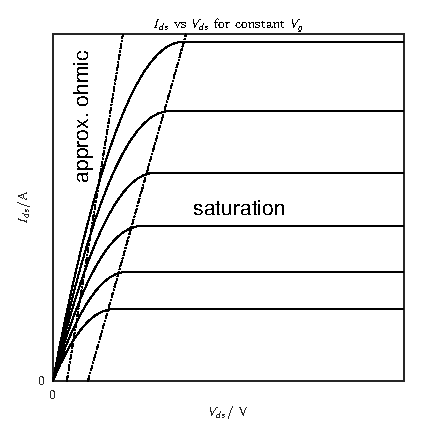
\includegraphics{prelab2.eps}
    \caption{Qualitative graphs of \(I_{ds}\) vs. \(V_{ds}\) in the above threshold region for varying \(V_g\).
    The ohmic and saturation regions are marked.}
    \label{fig:q2}
\end{figure}
The graphs of the drain currents for varying \(V_{ds}\) and \(V_g\) can be seen in Fig.~\ref{fig:q2}. These
differ from the equivalent graphs in subthreshold mode in that the saturation value of \(V_{ds}\) is not 
constant, but instead depends on the gate overdrive.

\subsection{Derive an expression for the current in the ohmic region, in terms of \(V_g\) and \(V_{ds}\)}
The general equation:
\begin{equation*}
    I_{ds} = \frac{\beta}{2}\left(\left(V_g-V_{T0}-V_s\right)^2-\left(V_g-V_{T0} - V_d\right)^2\right)
\end{equation*}
Can be reduced to 
\begin{equation*}
    I_{ds} = \beta\left(\left(V_g-V_{T0}\right)\left(V_d-V_s\right) - \frac{1}{2}\left(V_d-V_s\right)^2\right)
\end{equation*}
Replacing \(V_d-V_s = V_{ds}\) and assuming that \(V_{ds}\) is very small so the second term can be ignored we
have
\begin{equation*}
    I_{ds} = \beta V_{ds}\left(V_g-V_{T0}\right) 
\end{equation*}
A sketch of the current in the ohmic region can be seen in Fig.~\ref{fig:q3}. The current is proportional to
\(\beta\) and \(V_{ds}\).
\begin{figure}
    \center
    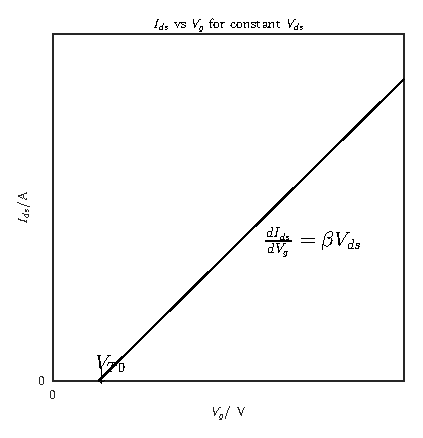
\includegraphics{prelab3.eps}
    \caption{\(I_{ds}\) versus \(V_g\) in the ohmic region.}
    \label{fig:q3}
\end{figure}

\subsection{State the drain voltage condition for above-threshold saturation and derive an expression for the saturation current, \(I_{dsat}\).}

The condition for saturation in the above threshold regime is \(V_{ds} \geq V_g - V_{T0}\).
When we are in saturation, there will be a pinchoff point under the channel with no electrons, therefore the
general equation reduces to 
\begin{equation*}
    I_{dsat} = \frac{\beta}{2}\left(V_g-V_{T0}\right)^2
\end{equation*}
Assuming \(\kappa = 1\). If the y-axis label in graph in Fig.~\ref{fig:q3} is replaced with \(\sqrt{I_{dsat}}\) and the slope replaced with a constant 
1, it shows the saturation current as a function of \(V_g\).

\subsection{Calculate \(C_{ox}\) for the classchip from the values given.}

The capacitance of a capacitor is 
\begin{equation*}
    C=\varepsilon\frac{A}{d}
\end{equation*}
When using the symbols used in the lab manual this becomes

\begin{equation*}
    C_{ox} = \varepsilon_{ox}\varepsilon_0\frac{WL}{t_{ox}}
\end{equation*}
We want the capacitance per square micron, so we calculate
\begin{equation*}
    \frac{C_{ox}}{WL} = \varepsilon_{ox}\varepsilon_0\frac{1}{t_{ox}} = 3.9\cdot8.86\cdot10^{-12}\frac{F}{m}\frac{1}{300\cdot10^{-10}m} = 0.0011518 \frac{F}{m^2} = 1.1518 \frac{fF}{\mu m^2}
\end{equation*}

\subsection{Write the expression for the drain current in saturation including the Early effect.}
The expression for the saturation current when taking the Early effect into account is
\begin{equation*}
    I = I_{dsat}+\left(1+\frac{V_{ds}}{V_E}\right)
\end{equation*}

\subsection{Sketch the setups you will use.}
\begin{figure}
    \begin{subfigure}{0.5\textwidth}
        \center
        \begin{circuitikz}[american voltages] \draw
            (0,0) node[nmos] (mos) {}
            (mos.base) node[anchor=west] {} -- (1,0) to[short] (1,-1)
            (1,-1) node[ground] {} (1,-1)
            (-1.5,-1) to[V] (-1.5,-0) -- (mos.gate)
            (mos.gate) node[anchor=east] {} 
            (-1.5,-1) node[ground] {} (-1.5,-1)
            (mos.drain) node[anchor=south] {} -- (0, 1) 
            (-2,1) to[V=$V_{d}$] (0,1)
            (-2,0.5) node[ground] {} to (-2,1) 
            (mos.source) node[anchor=north] {} to (0,-2)
            (0,-2) node[ground] {} to (0,-2)
            (-2,-0.5) node[anchor=east] {K230}
            (-0.6, 0.3) node[anchor=east] {K236}
        ;\end{circuitikz}
        \caption{}
    \end{subfigure}
    \begin{subfigure}{0.5\textwidth}
        \center
        \begin{circuitikz}[american voltages] \draw
            (0,0) node[pmos] (mos) {}
            (mos.base) node[anchor=west] {} -- (1,0) to[short] (1,1)
            (1,1) node[rrail] {} (1,1)
            (mos.gate) -- (-1.5,0) to[V] (-1.5,1) node[rrail] {}
            (mos.gate) node[anchor=east] {} 
            (mos.source) node[anchor=south] {} -- (0, 1)
            (0,1) node[rrail] {}
            node[right] {$V_{dd}$}
            (2,1) node[rrail] {} to[short] (2,-2) to[short] (0,-2)
            %(0,-2.0) to[V=$V_d$] (mos.drain)
            (mos.drain) to[V_=$V_d$] (0,-2)
            (-2,0.5) node[anchor=east] {K230}
            (+1.4, -1.5) node[anchor=east] {K236}
        ;\end{circuitikz}
        \caption{}
    \end{subfigure}
    \caption{Experimental setup for both pMOS and nMOS transistors that can be used in all three experiments. The TRIAX+ connector of the K236 is always
    connected to the transistor terminal.}
    \label{fig:setup1}
\end{figure}
Fig.~\ref{fig:setup1} shows the setups that will be used for all three experiments. The K236 is placed between the supply rail and drain terminal
of the pMOS in order to use the same rail for lower noise.

\end{document}
